%%
%  ******************************************************************************
%  * #file    Szablon_raportu_EN_Latex.tex
%  * #author  Adrian Wójcik   adrian.wojcik(at)put.poznan.pl
%  *          
%  * #commit  Patryk Kościk   koscikpatryk(at)gmail.com
%  *          Modified the template for Projekt przejsciowy purposes          
%  *          
%  * #version 1.0
%  * #date    09-Mar-2022
%  * #brief   PROJPRZEJ
%  *
%  ******************************************************************************
%%  
\documentclass[11pt, a4paper]{article}

\usepackage{SM_template}

% Wypełnijcie te dyrektywy zgodnie z waszym tematem
% \lab      -> NAZWA CZUJNIKA, np.: 'DHT22'
% \comment  -> Króciutki opis co to, np.: 'Cyfrowy budżetowy czujnik temperatury'
%

\lab{Moduł KY-018}
\comment{Analogowy czujnik natężenia światła}
\author{Dawid Wasung}
\addbibresource{bib/KY-018.bib}

% Absolutny zakaz dotykania tego tutaj bo jak dotkiecie to coś jebnie
\university{Politechnika Poznańska}
\faculty{Wydział Automatyki, Robotyki i Elektrotechniki}
\institute{Instytut Robotyki i Inteligencji Maszynowej}
\department{Zakład Sterowania i Elektroniki Przemysłowej}

\nocite{*}


%%
%
% Początek dokumentu
%
%%
\begin{document}

%% Strona tytułowa %%
\mainpage{{KY-018/foto}}
\newpage

\section*{Opis elementu} \addcontentsline{toc}{section}{Wstęp}
Czujnik KY-018 składa się z fotorezystora, wbudowanego rezystora 10k $\Omega$ oraz trzech pinów męskich. Fotorezystor jest elementem półprzewodnikowym, którego rezystancja ulega zmianie pod wpływem padającego na niego promieniowania elektromagnetycznego; przykładowo promieniowania widzialnego lub podczerwieni. Rezystancja elementu zależy od natężenia oświetlenia fotorezystora, jego rezystancja w ciemności jest bardzo duża i może osiągnąć wartość rzędu megaomów, przy silnym oświetleniu może zmaleć do kilku omów.
\vspace{0.5cm}
\begin{figure}[h!]
\centering
\begin{subfigure}{.5\textwidth}
  \centering
  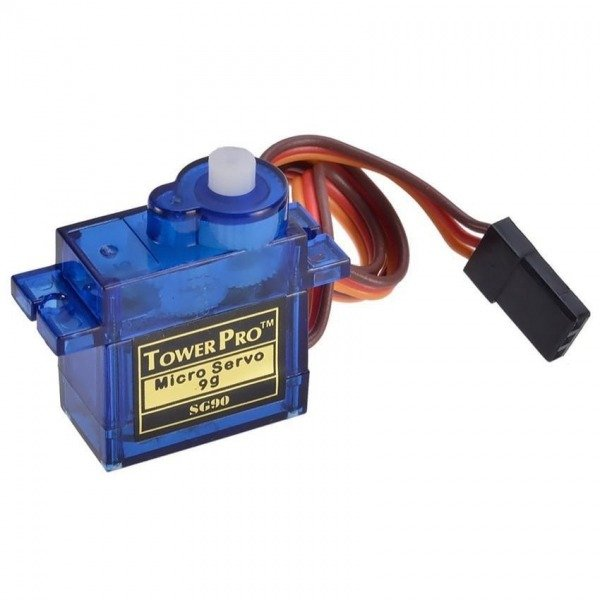
\includegraphics[width=.4\linewidth]{fig/KY-018/zdj_modułu/fig1.png}
  \caption{Moduł KY-018 \cite{ArduinoModules:Switch}}
  \label{fig:sub1}
\end{subfigure}%
\begin{subfigure}{.5\textwidth}
  \centering
  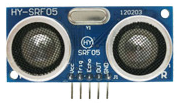
\includegraphics[width=0.737\linewidth]{fig/KY-018/zdj_modułu/fig2.png}
  \caption{Fotorezystor (THT) \cite{ArduinoModules:grab}}
  \label{fig:sub2}
\end{subfigure}
\caption{Poglądowe rysunki modułu oraz fotorezystora}
\label{fig:test}
\end{figure}

Fotorezystor posiada dwa wyprowadzenia oraz charakterystyczną powierzchnię światłoczułą, na której znaleźć można grzebieniowe elektrody podłączone do 2 wyprowadzeń. Fotorezystory są wykonywane z półprzewodnika (np. krzemu lub siarczku ołowiu), który naniesiony jest na szklane podłoże. Światło padające na czujnik generuje nośniki ładunku elektrycznego, co ułatwia przepływ prądu.

\begin{figure}[h!]
\centering
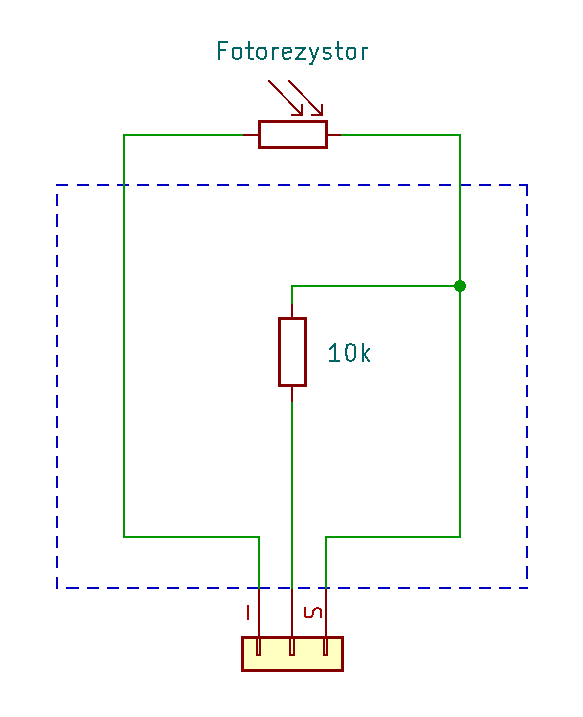
\includegraphics[width=.37\linewidth]{fig/KY-018/zasada_dzialania/schemacik.png}
\caption{Schemat modułu}
\label{fig:sub2}
\end{figure}

\newpage
\section*{Użycie czujnika}
Jako fotorezystory stosuje się półprzewodniki, które w temperaturze działania nie mają elektronów w paśmie przewodnictwa. Padające na półprzewodnik fotony o energii większej od przerwy energetycznej przemieszczają elektrony z pasma walencyjnego do pasma przewodnictwa, w wyniku którego powstają pary dziura-elektron, zjawisko nazywane jest efektem fotoelektrycznym wewnętrznym. W wyniku tego zjawiska następuje zwiększenie konduktancji materiału. Stosuje się je w aplikacjach, w któych konieczna jest kontrola obecności lub braku światła, przykładowo lamp nocnych, czy też do pomiaru jasności. 


Poniżej przedstawiono podstawową implementację czujnika na płytce stykowej.

\vspace{0.5cm}
\begin{figure}[h!]
    \centering
    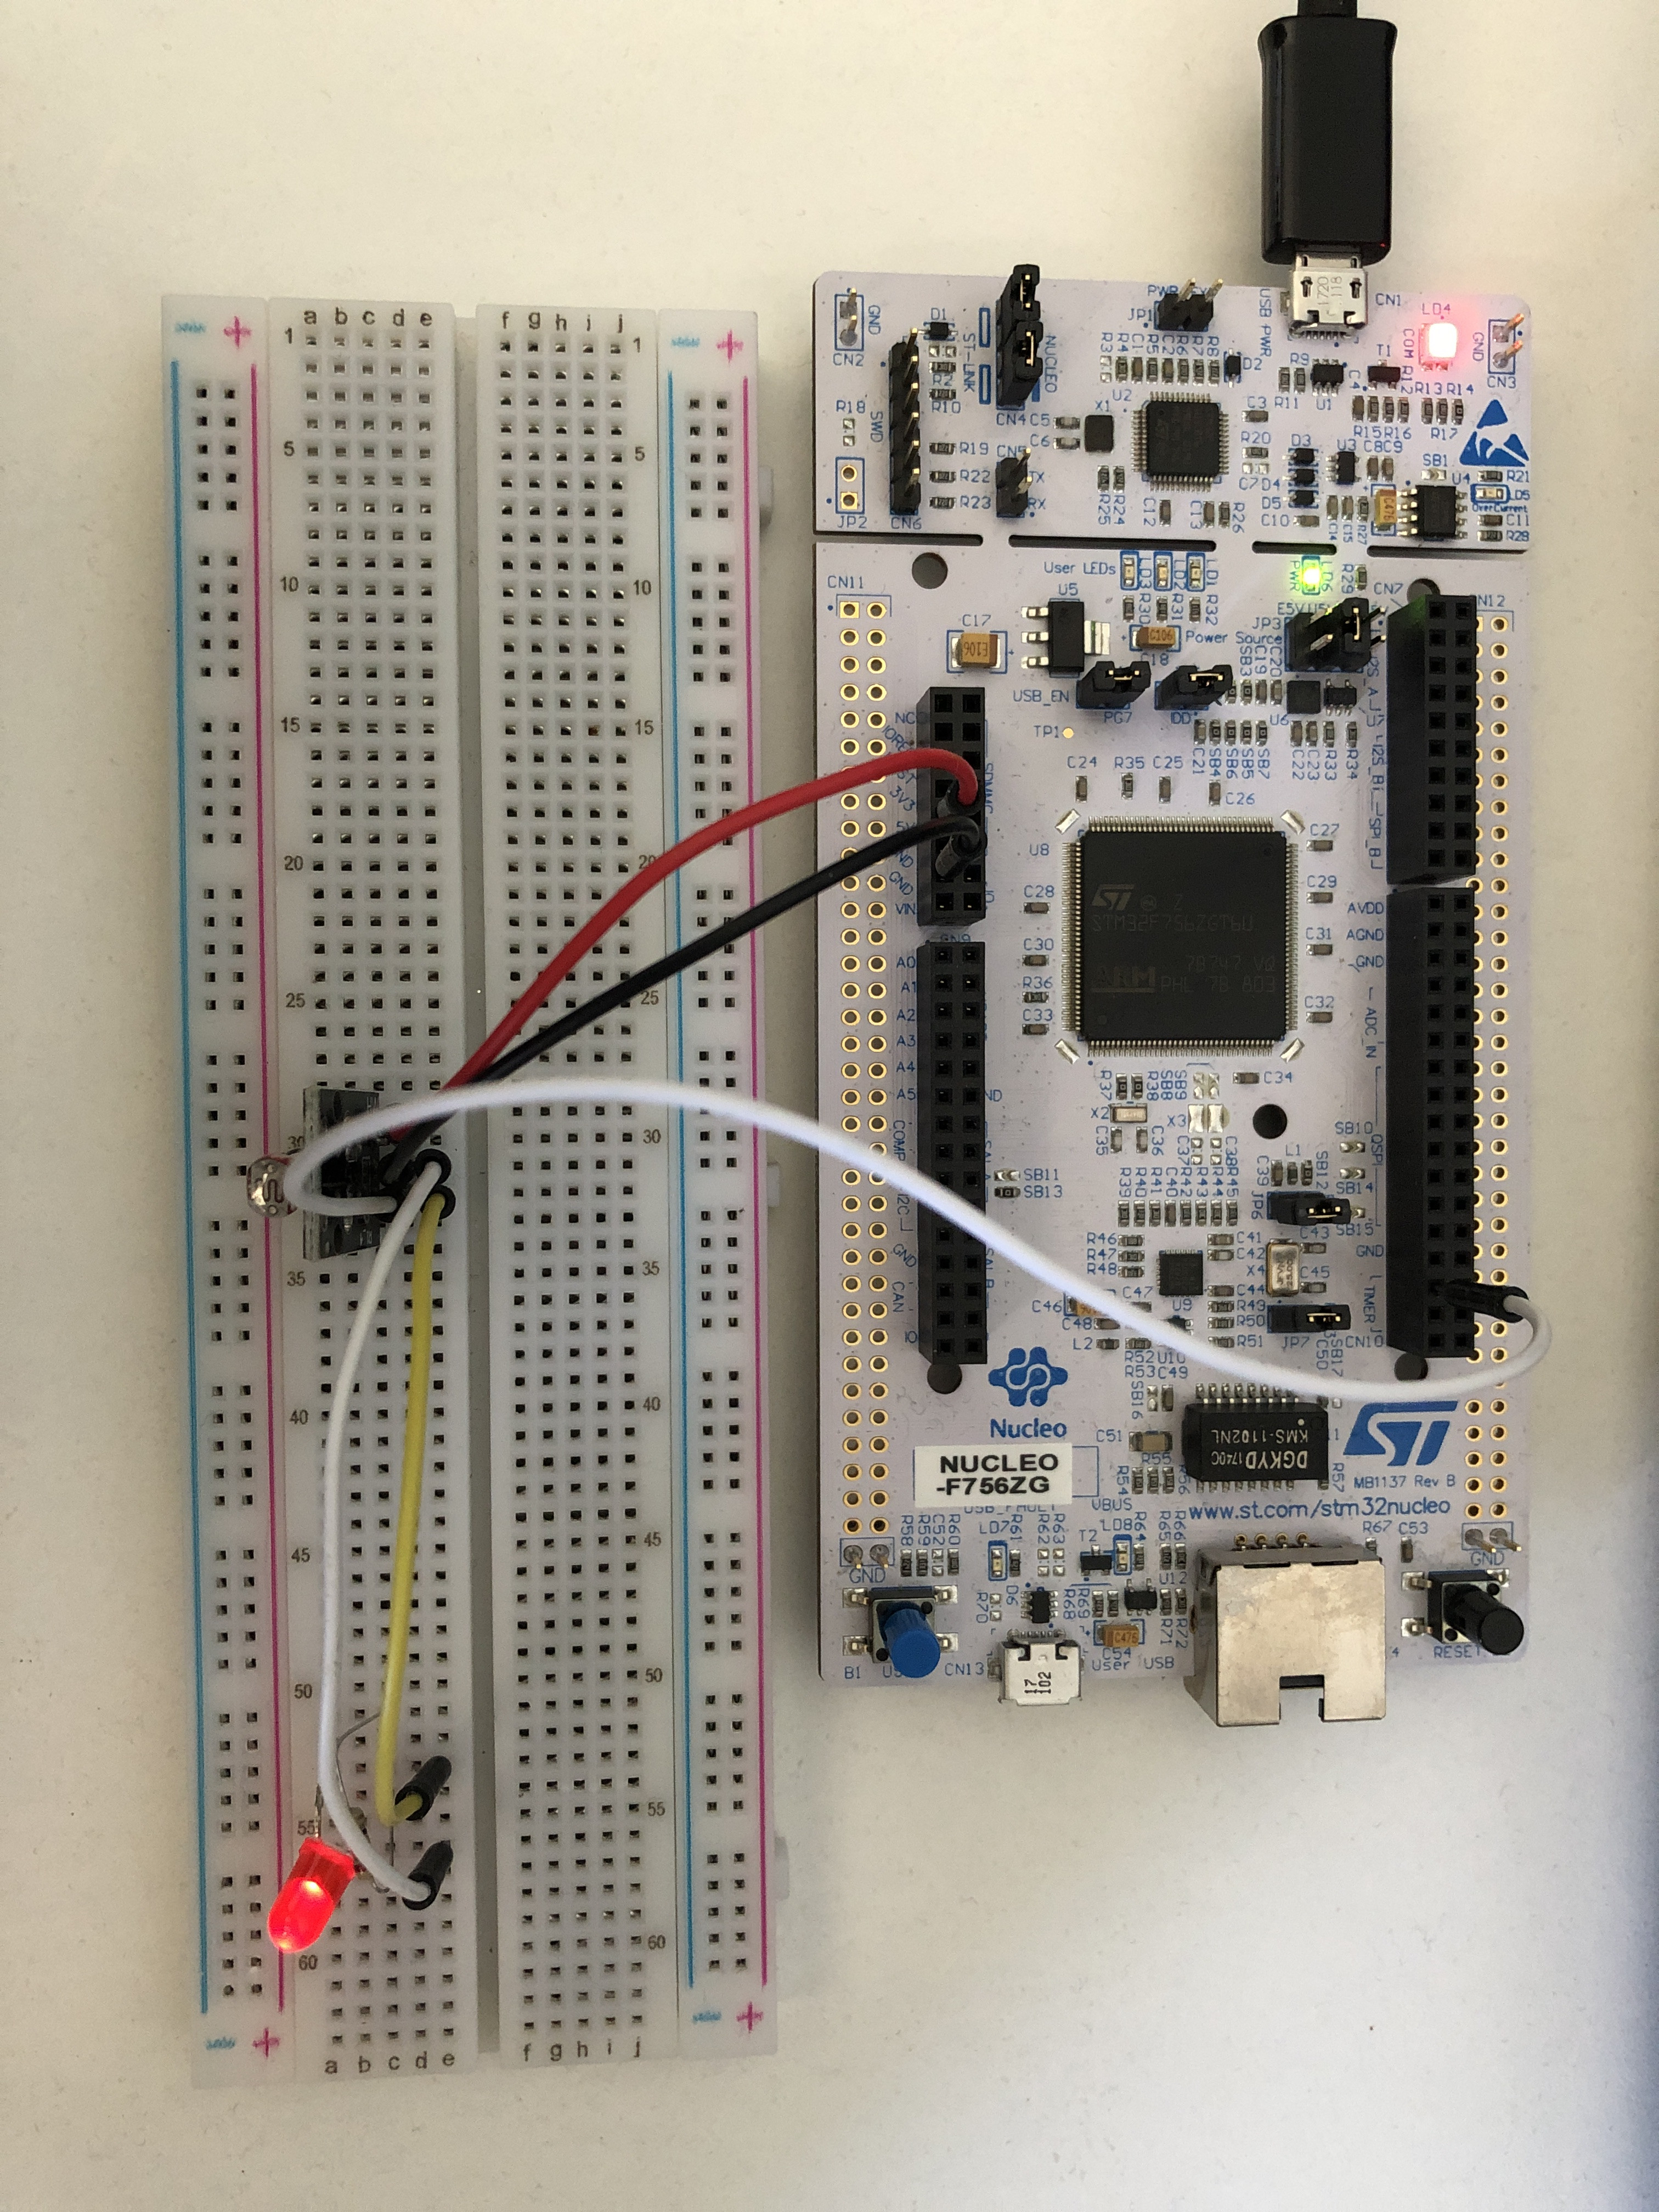
\includegraphics[width=0.45\textwidth,angle=90,origin=c]{fig/KY-018/działanie_ukladu/final.jpg}
    \caption{Działanie fotorezystora przy dużym natężeniu światła}
    \label{fig:my_label}
\end{figure}

Na Rys.3 widnieje zbudowany układ z modułem KY-018. Na fotorezystor pada światło dzienne, reyzstancja jest niska - dioda obrazująca działanie układu się świeci. W podanej implementacji czujnika zostało zamienione podłączenie pinów GND oraz napięcia, ze względu na odwróconą polaryzację przylutowanego fotorezystora (po podłączeniu według oznaczeń, fotorezystor działa na odwrotnej zasadzie - przy dużym natężeniu światła rezystancja jest mniejsza, niż przy niskim). 


\newpage
\begin{figure}[h!]
    \centering
    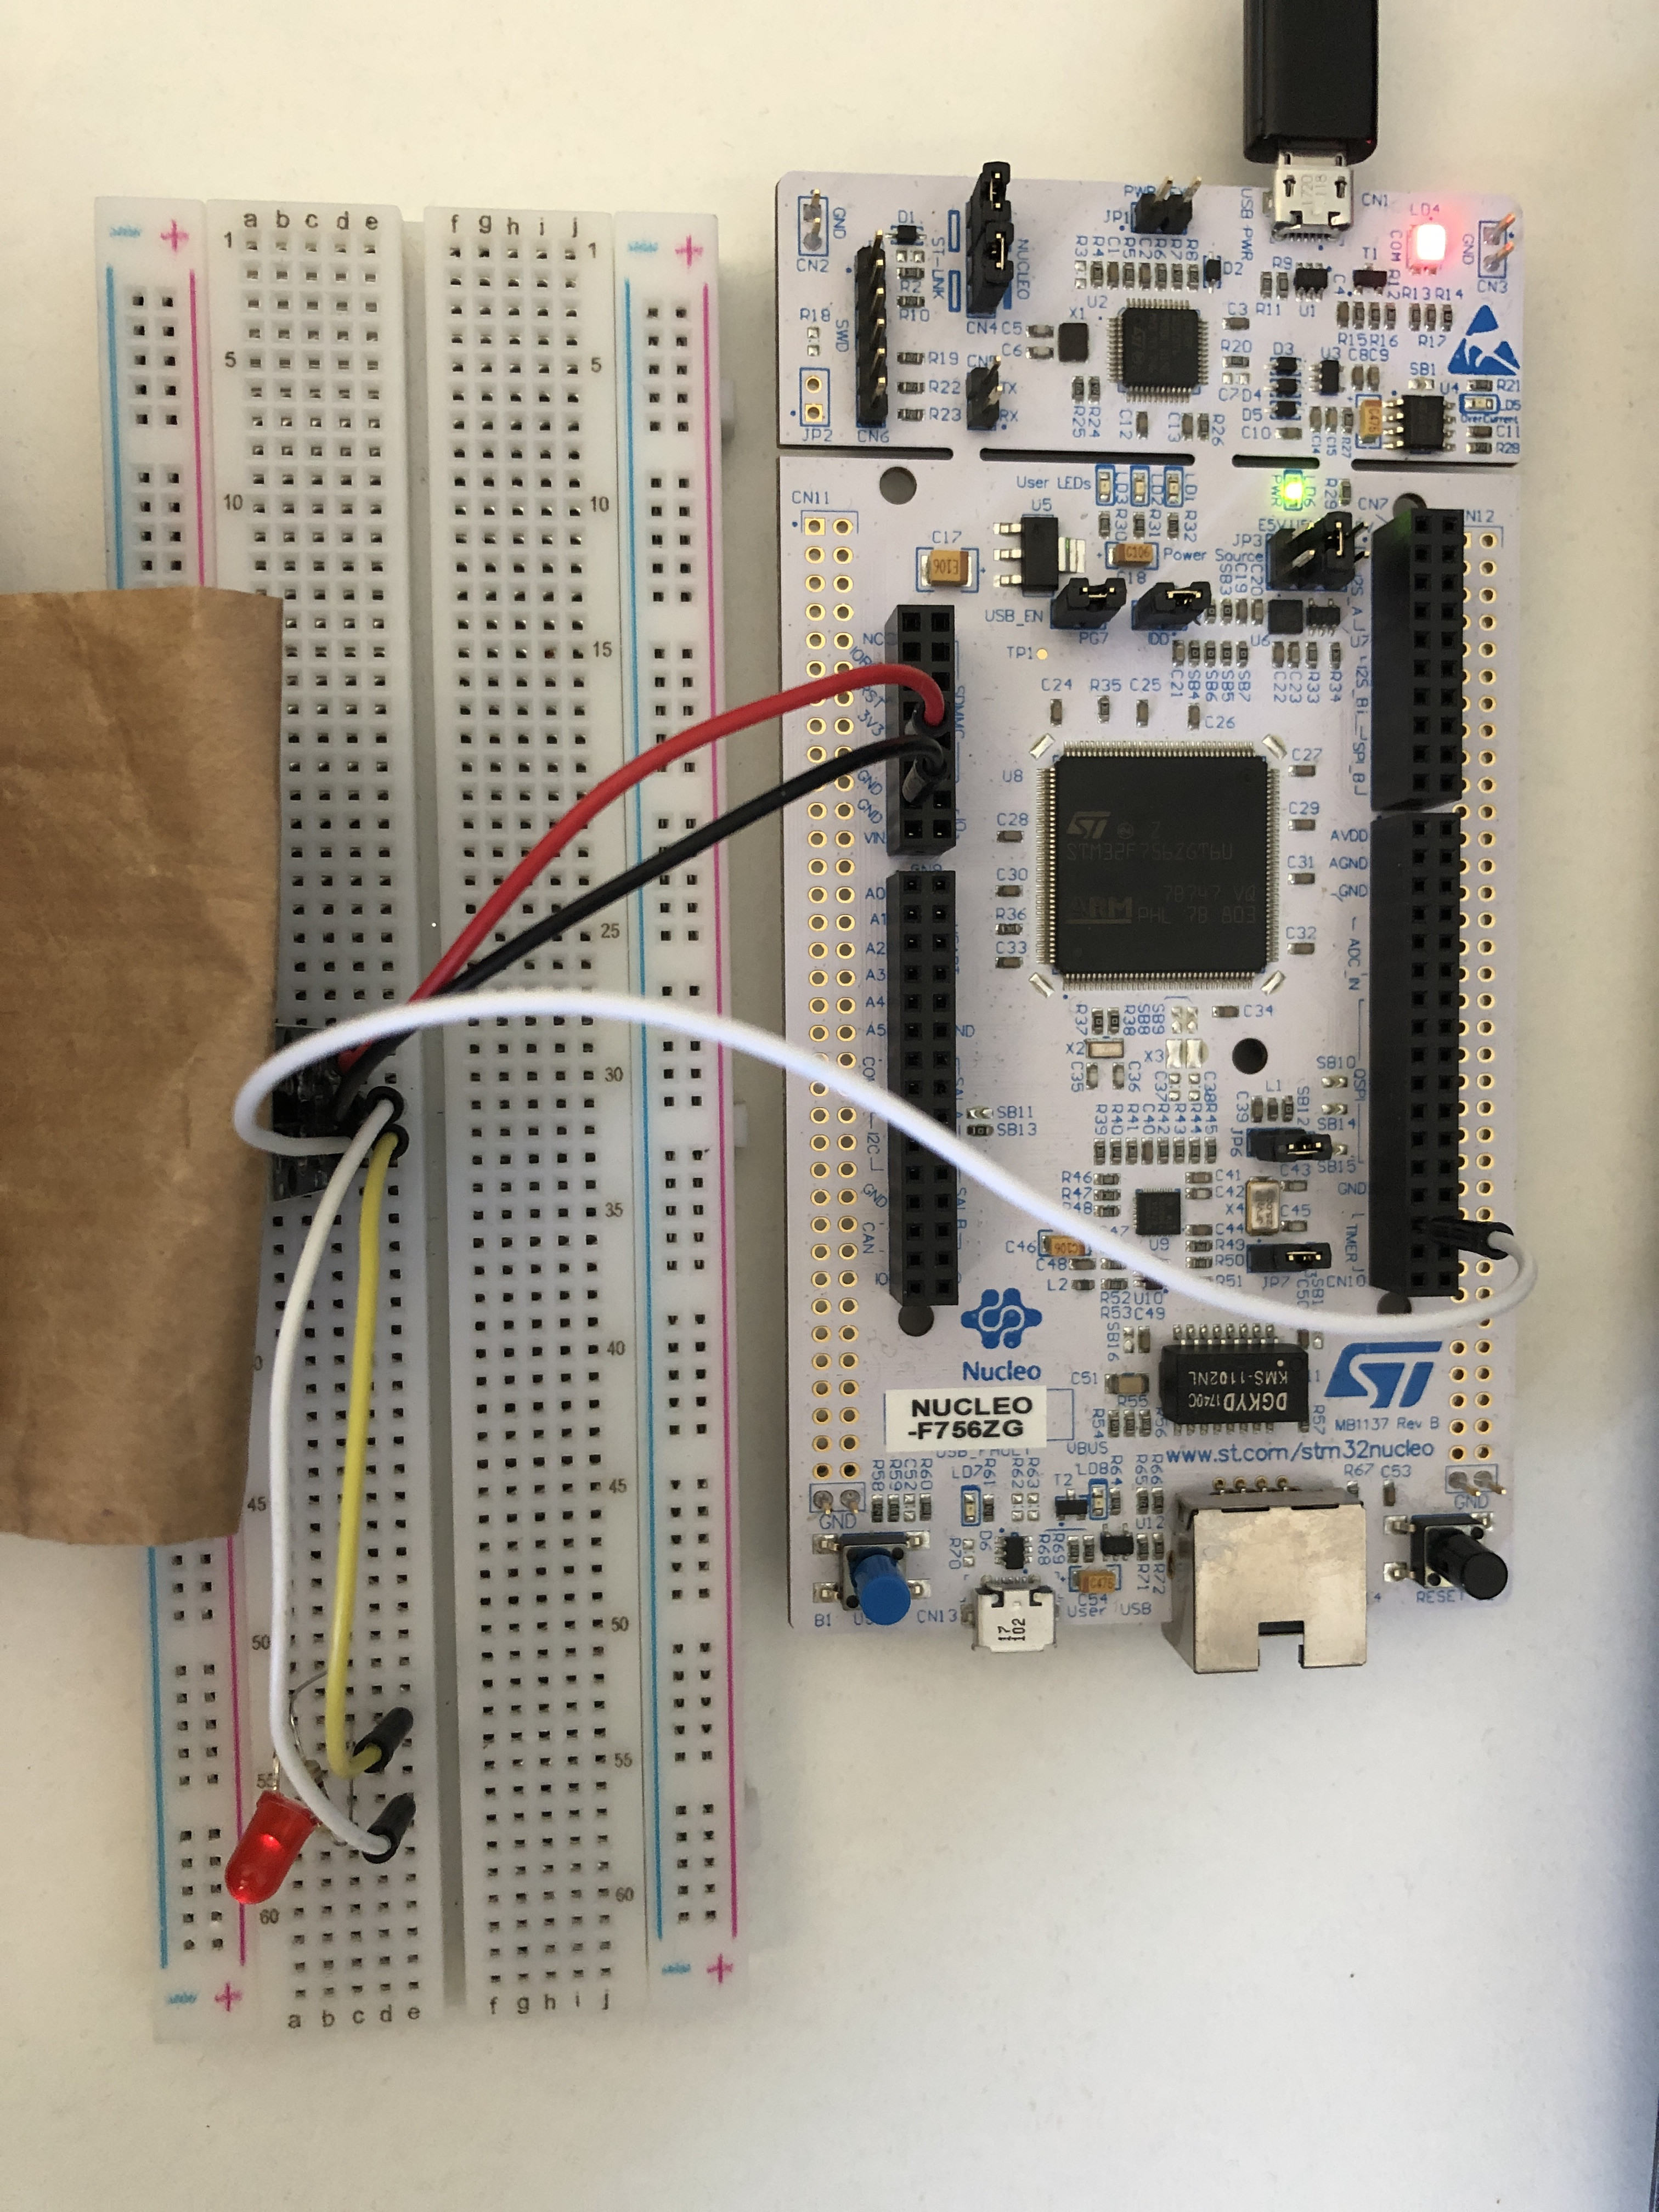
\includegraphics[width=0.45\textwidth,angle=90,origin=c]{fig/KY-018/działanie_ukladu/final2.jpg}
    \caption{Działanie fotorezystora przy małym natężeniu światła}
    \label{fig:my_label}
\end{figure}

Na Rys.4 fotorezystor został przykryty, co skutkuje zmniejszonym dostępem do zródła światła i tym samym - większej rezystancji. Dioda poglądowa świeci zdecydowanie słabiej niż na Rys.3, co obrazuje prawidłowe działanie czujnika.
\newline 



Kod programujący czujnik, wykorzystany do opracowania instrukcji, znajduje się w materiałach dodatkowych zawartych pod koniec rozdziału.
\newline
Film prezentujący działanie układu znajduje się w suplemencie wideo.
\printbibliography[heading=bibintoc]

\end{document}